\subsection{Geração de energia solar fotovoltaica}
\noindent Os modelos genéricos mais eficientes reduziram globalmente o consumo de energia elétrica, quando comparados com os modelos sem otimização, em cerca de 39,76\% para o modelo genérico otimizado mais eficiente, de 8 pavimentos, e 57,07\% para o modelo genérico otimizado mais eficiente, de 19 pavimentos. A partir destes resultados, foram selecionados os modelos mais eficientes entre os cenários simulados para cada tipologia e foram simuladas a implementação dos sistemas de produção de energia solar fotovoltaica.\vspace*{0.3cm} \newline
\noindent Observa-se que a energia elétrica gerada ao longo do ano, supriu a demanda de energia da edificação de 8 pavimentos para metade do ano e ligeiramente igualado em dois meses, abril e junho, como demonstrado no Gráfico 7. Anualmente, esta diferença é reduzida, produzindo maior energia do que a demanda anual, atingindo o balanço energético nulo, como apresentado no Gráfico 9. Nota-se, também, a proporção dos sistemas de condicionamento de ar – HVAC, iluminação e equipamentos em relação à produção de energia, correspondendo entre 30 a 40\% da composição do consumo para cada sistema avaliado. Os resultados com as configurações detalhadas dos equipamentos especificados estão descritos no Anexo I e II deste trabalho.
\begin{figure}[H]
    \centering
    \caption{Sistemas, consumo e produção de energia elétrica do modelo genérico de 8 pavimentos.}
    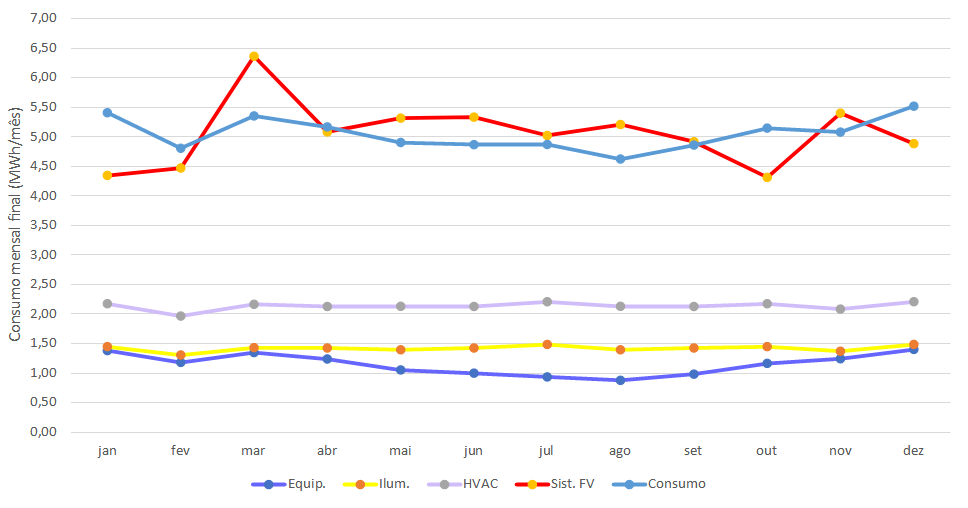
\includegraphics[width=1.0\textwidth]{figures/result/fig41-consumomod.png}
    \begin{flushleft}
        \par \small Fonte: autor, (2020).
    \end{flushleft}
    \label{fig:figure29}
\end{figure}
\noindent O desempenho do sistema de produção de energia fotovoltaica do modelo de 19 pavimentos atendeu à demanda anual. Nos meses de outubro e janeiro a demanda não foi correspondida, sendo quase nula a relação entre demanda e produção em dezembro, como observado no Gráfico 8. Observa-se que a proporção dos sistemas percebida no modelo de 8 pavimentos, em relação à produção de energia, é similarmente constatada neste modelo de 19 pavimentos.\vspace*{0.3cm} \newline
\noindent Os resultados de produção de energia para este modelo evidenciaram as características mais importantes para proporcionar maior geração de energia, como a área de fachada exposta a radiação solar e a relação entre a quantidade de pavimentos e a área de piso da edificação. Estes resultados de produção de energia em relação ao consumo foram importantes para indicar a potencialidade das edificações com dimensões como o modelo genérico proposto.
\begin{figure}[H]
    \centering
    \caption{Sistemas, consumo e produção de energia elétrica do modelo genérico de 19 pavimentos.}
    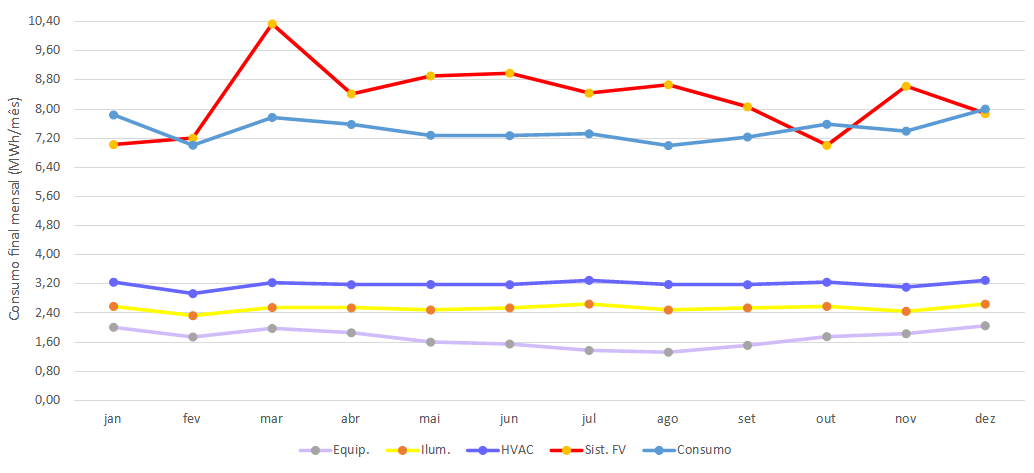
\includegraphics[width=1.0\textwidth]{figures/result/fig42-consumomod.png}
    \begin{flushleft}
        \par \small Fonte: autor, (2020).
    \end{flushleft}
    \label{fig:figure30}
\end{figure}
\vspace{-0.5cm} \noindent No Gráfico 9 e 14 são dispostas as médias mensais de consumo e produção de energia dos modelos genéricos otimizados de 8 e 19 pavimentos, respectivamente, assim como as médias anuais, as curvas tracejadas de média de produção de energia solar fotovoltaica e seus desvios padrões máximos e mínimos. Verificam-se os limites do sistema fotovoltaico para o modelo de 8 pavimentos, onde a relação quase nula entre geração e consumo de energia mensal é notada ao longo do ano simulado. Esta relação representa uma média anual de produção de energia superior ao consumo em 1,02\%, o que atesta o estado \textit{Zero Energy} para o modelo avaliado. Entretanto, a curva de desvio padrão mínimo mostra que em um cenário de pouca produção, o modelo seria dependente da energia fornecida pela concessionaria para atender as demandas mensais.\vspace{-0.3cm} 
\begin{figure}[H]
    \centering
    \caption{Consumo final mensal, Consumo vs. Produção de energia e Desvio Padrão das médias de produção de energia do modelo genérico otimizado de 8 pavimentos.}
    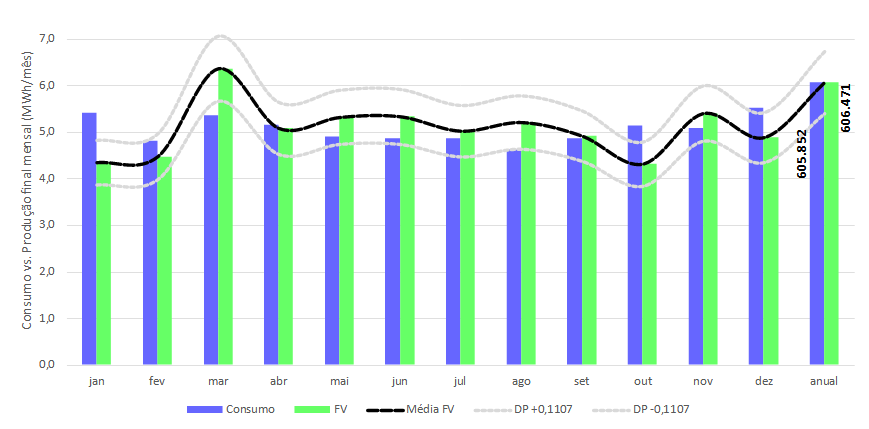
\includegraphics[width=1.0\textwidth]{figures/result/fig43-consumofinal.png}
    \begin{flushleft}
        \par \small Fonte: autor, (2020).
    \end{flushleft}
    \label{fig:figure31}
\end{figure}
\noindent Entretanto, para o cenário ótimo simulado para o modelo genérico otimizado de 19 pavimentos, percebe-se que não há a mesma dependência da Rede Pública para o fornecimento de energia. Este fato é constatado em um cenário onde a curva de desvio padrão mínimo seja a média de produção de energia do sistema sugerido, apresentando resultados superiores ao consumo na maior parte do ano.
\begin{figure}[H]
    \centering
    \caption{Consumo final mensal, Consumo vs. Produção de energia e Desvio Padrão das médias de produção de energia do modelo genérico otimizado de 19 pavimentos.}
    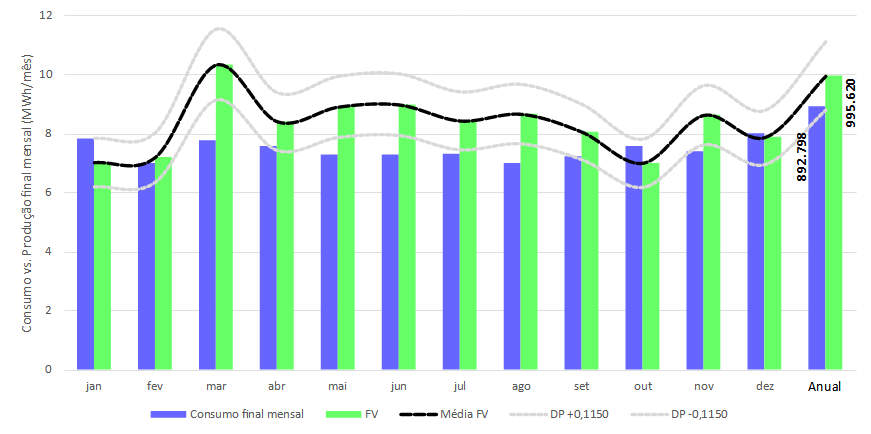
\includegraphics[width=1.0\textwidth]{figures/result/fig44-consumofinal.png}
    \begin{flushleft}
        \par \small Fonte: autor, (2020).
    \end{flushleft}
    \label{fig:figure32}
\end{figure}